%%%%%%%%%%%%%%%%%%%%%%%%%%%%%%%%%%%%%%%%%
% Beamer Presentation
% LaTeX Template
% Version 1.0 (10/11/12)
%
% This template has been downloaded from:
% http://www.LaTeXTemplates.com
%
% License:
% CC BY-NC-SA 3.0 (http://creativecommons.org/licenses/by-nc-sa/3.0/)
%
%%%%%%%%%%%%%%%%%%%%%%%%%%%%%%%%%%%%%%%%%

%----------------------------------------------------------------------------------------
%	PACKAGES AND THEMES
%----------------------------------------------------------------------------------------

\documentclass{beamer}

\mode<presentation> {

% The Beamer class comes with a number of default slide themes
% which change the colors and layouts of slides. Below this is a list
% of all the themes, uncomment each in turn to see what they look like.

%\usetheme{default}
%\usetheme{AnnArbor}
%\usetheme{Antibes}
%\usetheme{Bergen}
%\usetheme{Berkeley}
%\usetheme{Berlin}
%\usetheme{Boadilla}
%\usetheme{CambridgeUS}
%\usetheme{Copenhagen}
%\usetheme{Darmstadt}
%\usetheme{Dresden}
%\usetheme{Frankfurt}
%\usetheme{Goettingen}
%\usetheme{Hannover}
%\usetheme{Ilmenau}
%\usetheme{JuanLesPins}
%\usetheme{Luebeck}
\usetheme{Madrid}
%\usetheme{Malmoe}
%\usetheme{Marburg}
%\usetheme{Montpellier}
%\usetheme{PaloAlto}
%\usetheme{Pittsburgh}
%\usetheme{Rochester}
%\usetheme{Singapore}
%\usetheme{Szeged}
%\usetheme{Warsaw}

% As well as themes, the Beamer class has a number of color themes
% for any slide theme. Uncomment each of these in turn to see how it
% changes the colors of your current slide theme.

%\usecolortheme{albatross}
%\usecolortheme{beaver}
%\usecolortheme{beetle}
%\usecolortheme{crane}
%\usecolortheme{dolphin}
%\usecolortheme{dove}
%\usecolortheme{fly}
%\usecolortheme{lily}
%\usecolortheme{orchid}
%\usecolortheme{rose}
%\usecolortheme{seagull}
%\usecolortheme{seahorse}
%\usecolortheme{whale}
%\usecolortheme{wolverine}

%\setbeamertemplate{footline} % To remove the footer line in all slides uncomment this line
%\setbeamertemplate{footline}[page number] % To replace the footer line in all slides with a simple slide count uncomment this line

%\setbeamertemplate{navigation symbols}{} % To remove the navigation symbols from the bottom of all slides uncomment this line
}

\usepackage{graphicx} % Allows including images
\usepackage{booktabs} % Allows the use of \toprule, \midrule and \bottomrule in tables
\usepackage{multirow}
\newcommand{\xmark}{\textcolor{red}{\text{\sffamily X}}}
\newcommand{\cmark}{\textcolor{green}{\checkmark}}
\newcommand{\tr}{\text{tr}}
\newcommand{\E}{\textbf{E}}
\newcommand{\diag}{\text{diag}}
\newcommand{\argmax}{\text{argmax}}
\newcommand{\argmin}{\text{argmin}}
\newcommand{\Cov}{\text{Cov}}
\newcommand{\Vol}{\text{Vol}}

%----------------------------------------------------------------------------------------
%	TITLE PAGE
%----------------------------------------------------------------------------------------


\title{A practical evaluation of recent methods in high-dimensional inference}

\author{Charles Zheng} % Your name
\institute[Stanford] % Your institution as it will appear on the bottom of every slide, may be shorthand to save space
{Stanford University}
\date{\today} % Date, can be changed to a custom date

\begin{document}

\begin{frame}
\titlepage % Print the title page as the first slide
\end{frame}

\section{Introduction}

\begin{frame}
\frametitle{Theory and Practice}
\begin{center}
\begin{tabular}{c|c}
\underline{Theory} & \underline{Practice}\\
$Y \sim N(\beta' X, \sigma^2 I)$ & $Y, X_1,\hdots, X_p$ \emph{unknown} relationship
\end{tabular}
\end{center}
\end{frame}

\begin{frame}
\frametitle{Theory and Practice}
\begin{center}
\begin{tabular}{c|c}
\underline{Theory} & \underline{Practice}\\
$Y \sim N(\beta' X, \sigma^2 I)$ & $Y, X_1,\hdots, X_p$ \emph{unknown} relationship\\
$X_i = \begin{cases}
\text{non-null} & \beta_i \neq 0\\ 
\text{null} & \beta_i = 0
\end{cases}$ &
$X_i = \begin{cases}
\text{interesting}\\ 
\text{uninteresting}\\
\text{???}
\end{cases}$
\end{tabular}
\end{center}
\end{frame}

\begin{frame}
\frametitle{Methods}
\textcolor{white}{But what's actually used in practice?}
\begin{center}
\begin{tabular}{c|c|c|c|c}
 & Control & $p \leq n$ &  $p > n$\\ \hline
Classical inference (Pearson 1930) & Marginal & Yes & \\ \hline
Covariance test (Lockhart et al. 2014) &  ? & Yes & Yes\\ \hline
Debiased lasso (Javanmard et al. 2014) & Marginal & & Yes\\ \hline
Knockoffs (Barber et al. 2014) & FDR & Yes & ? \\ \hline
 & & & \\ \hline
\end{tabular}
\end{center}
\end{frame}

\begin{frame}
\frametitle{Methods}
But what's actually used in practice?
\begin{center}
\begin{tabular}{c|c|c|c|c}
 & Control & $p \leq n$ &  $p > n$\\ \hline
Classical inference (Pearson 1930) & Marginal & Yes & \\ \hline
Covariance test (Lockhart et al. 2014) &  ? & Yes & Yes\\ \hline
Debiased lasso (Javanmard et al. 2014) & Marginal & & Yes\\ \hline
Knockoffs (Barber et al. 2014) & FDR & Yes & ? \\ \hline
\textbf{Marginal screening} & ? & Yes & Yes \\ \hline
\end{tabular}
\end{center}
\end{frame}

\begin{frame}
\frametitle{Regression vs Marginal Screening}
\begin{itemize}
\item<1-> Why not just test $H_i: \Cov(X_i, Y) \neq 0$?
\item<1-> \emph{Even if} $Y = X\beta + \epsilon$, most non-null $X_i$ are probably also correlated
\item<2> In ``big data'' \emph{many} $X_i$ are correlated to $Y$, but \emph{redundant}
\end{itemize}
\end{frame}

\begin{frame}
\frametitle{Regression vs Marginal Screening}
Genome-wide association study
\begin{center}
\begin{tabular}{cc}
\multirow{5}{*}{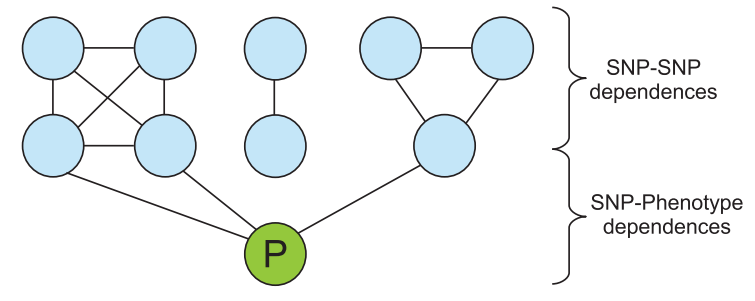
\includegraphics[scale = 0.3]{pgm.png}} & \\
& $\beta_i = 0$\\
& \vspace{0.2in}\\
& $\beta_i \neq 0$\\
& \vspace{0.2in}\\
\end{tabular}
\end{center}
(Adapted from \emph{Mourad 2012})
\end{frame}

\begin{frame}
\frametitle{From theory to practice}
\emph{Theory}
\begin{itemize}
\item<1-> Theory of inference in linear model
\item<3-> Theory of robust inference
\item<4-> Simulation studies
\item<5-> Validation on real data + \textbf{synthetic negative controls}
\item<2-> Validation of given procedure in real data with ground truth
\end{itemize}
\emph{Practice}
\end{frame}

\begin{frame}
\frametitle{Practical Validation}
\begin{itemize}
\item Difficult to validate inference procedures, because we would need to know the `\emph{true}' $\beta$
\item What is the `true' $\beta$ when the linear model is incorrect? We take
\[
\beta = \E[x x^T]^{-1} \E[yx]
\]
(the `superpopulation' model)
\item We don't know the ground truth in real data... what's the next best thing?
\end{itemize}
\end{frame}

\begin{frame}
\frametitle{Idea}
I give you real data \emph{mixed in} with noise variables
\begin{center}
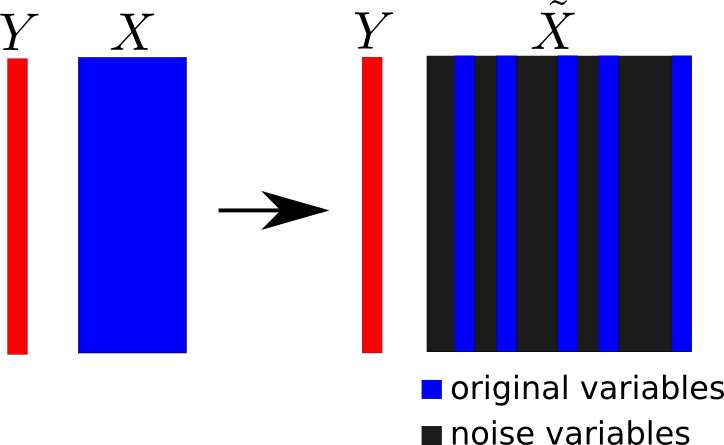
\includegraphics[scale = 0.35]{anc.png}
\end{center}
\begin{itemize}
\item Can you identify the original columns from the noise columns?
\item I can test your procedure this way, because I know the ground truth!
\end{itemize}
\end{frame}

\begin{frame}
\frametitle{Synthetic Negative Controls}
\begin{itemize}
\item<1-> Given random vector $x \in \mathbb{R}^p$, \emph{define} $\tilde{x} \in \mathbb{R}^{p+q}$ by
by
\[
\tilde{x} = \begin{pmatrix}I \\ \Gamma\end{pmatrix} x + e
\]
where $\Gamma$ is a fixed matrix and $e \perp x, y$.
\item<2-> Let
\[
\beta = \E[xx^T]^{-1}\E[yx], \ \ \tilde{\beta} = \E[\tilde{x}\tilde{x}^T]^{-1} \E[y\tilde{x}]
\]
\item<3-> Then
\[
\forall i \in \{1, \hdots, p\}: \beta_i = \tilde{\beta}_i
\]
\[
\forall i \in \{p+1,\hdots, p+q\}: \tilde{\beta}_i = 0
\]
\item<4->
\emph{Special case.} $X_{p+1},\hdots, X_{p+q}$ are pure noise: this is when $\Gamma = 0$
\end{itemize}
\end{frame}

\begin{frame}
\frametitle{Using SNCs to investigate robustness}
\begin{itemize}
\item<1-> All methods considered depend on strong assumptions (e.g. linearity, Gaussian iid errors, sparsity)
\item<1-> How well do these methods work on real data where assumptions are most likely violated?
\item<2-> Take low-dimensional real data mixed with SNCs (synthetic negative controls): can we identify the real data while controlling Type I error (measured by rejections of SNCs)?
\end{itemize}
\end{frame}

\begin{frame}
\frametitle{What can we conclude?}
\begin{itemize}
\item Experiments using SNCs shows that we can do well on the
  \emph{hypothesis testing problem} in realistic settings, where
  assumptions are violated
\item However, these experiments cannot tell us if we are solving the right problem!
\item Is the \emph{hypothesis testing problem} even relevant
  for the application? The only way to tell is validation on real,
  high-dimensional data with application-specific ground truth.
\end{itemize}
\end{frame}

\begin{frame}
\frametitle{Closing thoughts}
\begin{quotation}
``Statistics is a science in my opinion... for if its methods fail the
  test of experience -- not the test of logic -- they are discarded.''
\end{quotation}
\begin{quotation}
`` Both the statistician and the client must learn to confront the
  uncertainties of the world more explicitly, ... never to avoid
  responsibility for an ever-present understanding that all
  assumptions underlying data analysis are always approximations.
  Above all, they must base their thinking on a recognition that their
  assumptions will always require review and reappraisal...  ''
\end{quotation}
\hfill -- John Tukey
\end{frame}

\begin{frame}
\frametitle{References}
\begin{itemize}
\item Barber, R., and Candes, E. (2014). Controlling the False Discovery Rate via Knockoffs. arXiv Preprint arXiv:1404.5609, 1–27. Retrieved from http://arxiv.org/abs/1404.5609
\item Javanmard, A., and Montanari, A. (2014). Confidence intervals and hypothesis testing for high-dimensional regression. The Journal of Machine Learning Research, 15, 2869–2909. Retrieved from http://dl.acm.org/citation.cfm?id=2697057
\item Lockhart, R., Taylor, J., Tibshirani, R. J., and Tibshirani, R. (2014). a Significance Test for the Lasso. Annals of Statistics, 42(2), 413–468. doi:10.1214/13-AOS1175
\end{itemize}
\end{frame}


\begin{frame}
\frametitle{Acknowledgements}
Thanks to Will Fithian for useful discussions.
\end{frame}

\end{document}








\[
X = [1 | X_1 | \hdots | X_p] = \begin{pmatrix}x_1^T \\ \vdots \\ x_n^T \end{pmatrix}, \ \ Y = \begin{pmatrix}y_1 \\ \vdots \\ y_n \end{pmatrix}
\]
and
\[
\tilde{X} =  [X | X_{p+1} | \hdots | X_{p+1}] = 
\begin{pmatrix}\tilde{x}_1^T \\ \vdots \\ \tilde{x}_n^T \end{pmatrix}
\]
Let


